\documentclass[lnicst]{svmultln}
\usepackage{amssymb}
\usepackage{amsmath}
\setcounter{tocdepth}{3}
\usepackage{graphicx}
\usepackage{circuitikz}
\usepackage{listings}

\usepackage{tikz}
\usepackage{pgfplots}
\usepackage{pdflscape}
\usepackage{pgf}
\usepackage{pgfplotstable}
\usetikzlibrary{positioning, shapes.geometric, arrows, automata, pgfplots.groupplots}

\usepackage{url}
\urldef{\mailsa}\path|{mehari.msgna.2011, k.markantonakis, k.mayes}@rhul.ac.uk|
\usepackage[pdfpagelabels,hypertexnames=false,breaklinks=true,bookmarksopen=true,bookmarksopenlevel=2]{hyperref}

\definecolor{commentColor}{HTML}{21610B}


\begin{document}


\title{The B-Side of Side Channel Leakage: Control Flow Security In Embedded Systems}

\titlerunning{Control Flow Security In Embedded Systems}

\author{Mehari Msgna, Konstantinos Markantonakis, Keith Mayes}
				
\authorrunning{M. Msgna, K. Markantonakis, K. Mayes}

\institute{Smart Card Centre, Information Security Group, \\
		Royal Holloway, University of London, \\
		Egham, TW20 0EX, UK,\\
		\mailsa
}

\maketitle

\vspace{1cm}
\begin{abstract}
The security of an embedded system is often compromised when a ``trusted'' program is subverted to behave differently. Such as executing maliciously crafted code and/or skipping legitimate parts of a ``trusted'' program. Several countermeasures have been proposed in the literature to counteract these behavioural changes of a program. A common underlying theme in most of them is to define security policies at the lower level of the system in an independent manner and then check for security violations either statically or dynamically at runtime. In this paper we propose a novel method that verifies a program's behaviour, such as the control flow, by using the device's side channel leakage.

\keywords{Side Channel Leakage, Power Consumption, Program's Control Flow, Hidden Markov Model, Principal Components Analysis, Linear Discriminant Analysis}
\end{abstract}

\section{Introduction}
\label{sec:introduction}

In recent years, embedded systems have been proliferated into wide range of modern life applications. One of the main application vector of embedded systems is communication \cite{IET-12-AMMBPF,IEEE-12-A,ACM-11-AHS}. A typical embedded system application contains hardware and software components. The hardware component includes storage area, execution engine and other peripherals required to successfully execute instructions. The software component is a written procedures or rules stored in a memory pertaining to the operation of a computer system or part of the system itself.

The execution of a software program always involves incrementing the program counter (a special register which stores the address of the next instruction). Normally the program counter is incremented by ``1''; however, certain instructions change its value by more than one in both directions. This kind of change is known as \emph{Control Flow Change} and can be caused by both conditional and unconditional branching instructions. According to \cite{DAES-08-ST}, program control flow is the most attacked target in software and such attacks are called \emph{Control Flow Attacks}. \emph{Control Flow Attack} is one of the main threats for embedded systems \cite{CARDIS-11-GJJ,ACM-08-AC,SECWEST-13-D}. \emph{Control Flow Attacks} can be performed on embedded systems for two reasons. Firstly, the attacker installs his code segment on the target device. Then later when the device executes a genuine program, the attacker targets saved function return addresses to divert the control flow into his previously installed code. Secondly, the attacker does not install any code but instead when the program is executed the attacker changes the saved return addresses just in order to skip the execution of certain part of the program.

In the literature, several countermeasures have been proposed to counteract these kinds of intrusions. To explain some of them; in \cite{IEEE-06-DSAN}, the authors discuss a technique that employs a dedicated hardware module to detect and prevent unintended program behaviors. In this method the program's properties are extracted through a static code analysis and the hardware module uses them to enforce a permissible program behavior at runtime. Another countermeasure, described in~\cite{ACM-09-MMUJ} introduces \emph{Control-Flow Integrity (CFI)} enforcement. The CFI dictates that software execution must follow the path of a \emph{Control-Flow Graph (CFG)} determined ahead of time. The work of Michael Frantzen and Michael Shuey~\cite{USENIX-01-MM}, presents a buffer overflow prevention method. This is acheived via a kernel modification that performs transparent, automatic and atomic operations on the function return addresses before they are written into the stack and before the program transfers execution back to the saved return addresses. In \cite{ACM-09-ADC}, Aur{\'e}lien et al. discussed a control flow enforcement technique based on Instruction Based Memory Access Control (IBMAC). This is done by using a simple hardware modification to divide the stack into a data and a control flow stack (or return stack). Moreover, access to the control flow stack is restricted only to return and call instructions, which prevents control flow manipulation. More countermeasures can be found in \cite{ACSAC-06-CJCJP,USENIX-98-CCDHJPSAPQ,ASPLOS-04-GJDS}. Most of the proposed countermeasures are demanding in terms of computational capability, memory usage and often rely on a hardware module that is not present on simple devices.

In this paper we present a novel approach to verify a program's control flow by using the device's side channel leakage. In our proposal we modelled the device as a \emph{Markov Process} with hidden states, each state belonging to a part of the program. Then a verifying device extracts the control flow transition that the device had followed when executing the program from its side channel leakage (power consumption). This extracted control flow (state sequence) is then verified against a list of valid state transitions of the application which was calculated ahead of time.

The rest of the paper is structured as follows. Section~\ref{sec:power-analysis} briefly provides background information on side channel leakage. Section~\ref{sec:control-flow-verification} discusses the proposed control flow verification methodology. Section~\ref{sec:experiment} discusses our experimental results. Finally, section \ref{sec:conclusion} concludes the paper.

\section{Side Channel Leakage}
\label{sec:power-analysis}

Side channel leakage is information revealed by a device about its internal state while processing a certain procedure. Smart cards and other embedded devices use electric current to turn transistors on and off. The instantaneous electric current that the device consumes depends on how many transistors that the executed instructions and data turn on and off. This difference in the electric current is then reflected in the power consumption and electromagnetic emission of the device. The power consumption and/or electromagnetic emission can then be recorded and analysed to extract secret information from the target device.

In the context of cryptology, side channel leakage can be employed in retrieving cryptographic secret keys from target devices, such as smart cards. Side channel information such as timing \cite{CRYPTO-96-P,CARDIS-98-DKLMQ,CT-RSA-13-CP}, power consumption \cite{CRYPTO-99-PJB,IDaTC-07-TSE,CHES-11-DC} and electromagnetic emission \cite{CT-RSA-12-JSBFG,CIS-11-KLXX,CS-85-WN} have been used in attacking implementations of cryptographic algorithms including AES~\cite{AES-02-JV}, DES~\cite{DES-98-W} and RSA~\cite{ACM-78-RSA}.

Besides extracting cryptographic keys, side channel information has also been used to reverse engineer embedded device applications \cite{WISTP-07-DMG,TCS-10-TCB,IACR-04-C}. This is done by constructing a power consumption template of the target device using an identical reference device. Then use the templates to recognise executed instructions from the target device's power consumption waveform. In addition, side channel information can also be used by device manufacturers and application developers to detect cloned devices and design advanced applications. Instruction-level power consumption model of an embedded device has been used to design a low-power consuming applications for mobile embedded devices where batteries are the main power source \cite{LCTES-01-SASN,IEEE-04-NPSC}. In \cite{ACT-06-KKC}, the authors discuss, theoretically, how side channel leakage can be used to fingerprint a smart card platform and then use it later to detect cloned cards.

\section{Control Flow Verification}
\label{sec:control-flow-verification}

An application is a combination of basic blocks. A basic block is a linear sequence of executable instructions with only one entry point (the first instruction executed) and one exit point (the last instruction executed) \cite{SIGPLAN-70-F}. After executing one basic block the processor jumps into another basic block based on the branching instruction executed at the end of the current basic block. This branching instruction can be conditional or unconditional. A basic block may have many predecessors and many successors. It might also be its own successor. Program entry basic blocks might not have predecessors that are within the program and program ending basic blocks never have successors within the program itself.

An embedded device, with one or two programs installed in its non-volatile memory, can be modelled as a state machine with each state corresponding to a basic block of the program(s). When the program is being executed we can not directly observe the states that the processor is going through but we can observe the side channel information emitted by the device. Such information can be the power consumption \cite{CRYPTO-99-PJB,IDTC-07-TSE} or the electro-magnetic emission \cite{CIS-11-KLXX,CT-RSA-12-JSBFG,CS-85-WN} of the device. The side channel information emitted by the device is directly dependent on the states executed by the  processor.

The question here are, by only using this observable physical emission can we reconstruct the state sequence that the processor went through when executing the program? And once the sequence is reconstructed can we verify it?

\subsection{Control Flow Reconstruction}
\label{subsec:reconstruction}

To reconstruct the state sequence that a device followed during the execution of a program from its side channel leakage we modelled the device as a \emph{Hidden Markov Model (HMM)} \cite{Book-08-F,IEEE-89-L}. A \emph{Markov Model} is a memoryless system with a finite number of hidden states. It is called memoryless because the next state depends only on the current state.

In such model the states are not directly observable. However, there has to be (at least) one observable output of the process that reveals partial information about the state sequence that the device has followed. Fig.~\ref{fig:hmm-model-processor}, illustrates a \emph{Markov Process} with five hidden states (i.e A to E).

\begin{figure}[ht!]
	\centering
	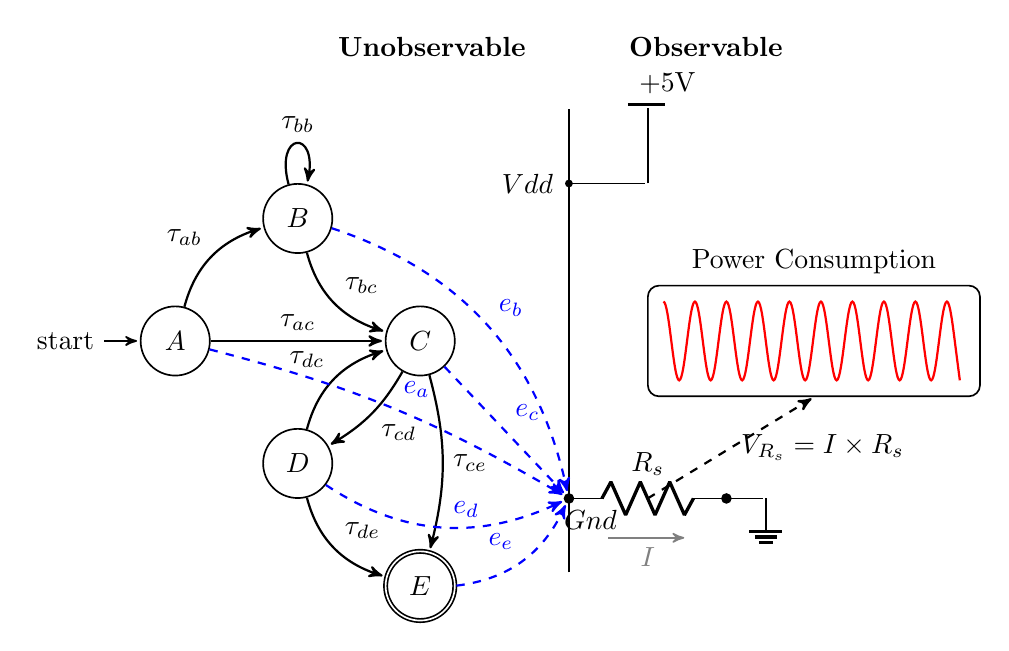
\begin{tikzpicture}[>=stealth', shorten >=1pt, auto, node distance=2.2cm, semithick,
											dot/.style={circle,inner sep=1pt,fill,name=#1},
  										extended line/.style={shorten >=-#1,shorten <=-#1},
  										extended line/.default=1cm,
  										block/.style={rectangle,draw, text centered, rounded corners, minimum height=4em, minimum width=12em}]
  										
	  \tikzstyle{every state}=[fill=white, draw=black, text=black]
	
	  \node[initial,state] (A)                    {$A$};
	  \node[state]         (B) [above right of=A] {$B$};
	  \node[state]         (D) [below right of=A] {$D$};
	  \node[state]         (C) [below right of=B] {$C$};
	  \node[state,accepting]   (E) [below right of=D] {$E$};

	  \path[->,thick] (A) edge [bend left]  node {$\tau_{ab}$} (B)
	                      edge              node {$\tau_{ac}$} (C)
						        (B) edge [loop above] node {$\tau_{bb}$} (B)
						            edge [bend right]  node {$\tau_{bc}$} (C)
						        (C) edge [bend left=15pt]  node {$\tau_{cd}$} (D) 
						            edge [bend left=15pt]  node {$\tau_{ce}$} (E)
						            
						        (D) edge [bend left] node {$\tau_{dc}$} (C)
						            edge [bend right] node {$\tau_{de}$} (E);
		
		\node [dot=GND] at (5,-2) {};
		\node (gnt-txt)   [below right of=GND, node distance=1.1em] {$Gnd$};
		\node [dot=Vdd] at (5, 2) {};
		\node (vdd-txt)   [left of=Vdd, node distance=1.5em] {$Vdd$};
		\draw [thick, extended line=1cm] (GND) -- (Vdd);
		
		\node (obs-text)   [above left of=Vdd, node distance=7em] {\textbf{Unobservable}};
		\node (unobs-text) [above right of=Vdd, node distance=7em] {\textbf{Observable}};
		
		\draw (GND) to[R=$R_{s}$,*-*] (7, -2);
		%Current across the resistor.
		\path[->] (5.5,-2.5) edge [gray] node[below, pos=0.5] {$I$} (6.5,-2.5);
		\draw (7, -2) --++(0.5,0) node[ground] {};
		
		\path[->, thick] (A) edge [bend left=8pt, blue, dashed]             node {$e_{a}$} (GND)
				             (B) edge [blue, bend left, dashed]  node {$e_{b}$} (GND)
				             (C) edge [blue, dashed]             node {$e_{c}$} (GND)
				             (D) edge [blue, bend right, dashed] node {$e_{d}$} (GND)
				             (E) edge [blue, bend right, dashed] node {$e_{e}$} (GND);
				             
		\node [block] (scope)   [right of=C, node distance=5cm] 	  {$ $};
		\node         (pc-text) [above of=scope, node distance=1cm] {Power Consumption};
		
		\draw [red, thick] (6.2,0.5) cos(6.3,0) sin(6.4,-0.5) cos(6.5,0) sin (6.6,0.5) cos (6.7,0) sin (6.8,-0.5) cos (6.9,0) sin (7.0,0.5) cos (7.1,0) sin (7.2,-0.5) cos (7.3,0) sin (7.4,0.5) cos (7.5,0) sin (7.6,-0.5) cos (7.7,0) sin (7.8,0.5) cos (7.9,0) sin (8.0,-0.5) cos (8.1,0) sin (8.2,0.5) cos (8.3,0) sin (8.4,-0.5) cos (8.5,0) sin (8.6,0.5) cos (8.7,0) sin (8.8,-0.5) cos (8.9,0) sin (9.0,0.5) cos (9.1,0) sin (9.2,-0.5) cos (9.3,0) sin (9.4,0.5) cos (9.5,0) sin (9.6,-0.5) cos (9.7,0) sin (9.8,0.5) cos (9.9,0) sin (10.0,-0.5);
		
		%Instantaneous voltage accross the resistor.
		\path[->, thick] (6,-2) edge [black, dashed] node[right, pos=0.5] {$V_{R_{s}}=I\times R_{s}$} (scope.south);
		\draw (5, 2)   --++ (1.0, 0);
		\draw (6, 2)   --++ (0, 1.0);
		\draw [very thick] (5.75, 3.0) --++ (0.5, 0) node[above] {+5V};
		
	\end{tikzpicture}
	\caption{A Markov model representing a device executing a program with five states (A, B, C, D and E). The power consumption is the observable output that reveals partial information about the state sequence of the device.}\label{fig:hmm-model-processor}
\end{figure}

In case of the \emph{Markov Process} illustrated in Fig.~\ref{fig:hmm-model-processor}, the hidden states are the program's basic blocks and the observable output is the power consumption of the device. This observable output is measured via a resistor ($R_{s}$) connecting the ground pin of the device and ground pin of the voltage source.

\subsubsection{Building The Hidden Markov Model}
\label{subsubsec:build-hmm}

Building a \emph{Hidden Markov Model (HMM)} requires a set of finite states $q_{i}$'s, a transition probability distribution matrix $\mathbf{T}=\{ \tau_{ij} \}$, emission probability distribution matrix $\mathbf{E}=\{ e_{i} \}$ and initial state distribution $\vec{\pi}$. Given these probability distribution matrices, the HMM is defined as $\lambda =(\mathbf{T},\mathbf{E},\vec{\pi})$.

The transition probability distribution $\tau_{ij}$, is the probability that the next state is $q_{j}$ if the current state is $q_{i}$, for $1 \leq i,j \leq S$ where $S$ is the number of states. If we denote $s_{t}$ the current state of the system at a time $t$, $\tau_{ij} = \mathcal{P}(s_{t+1}=q_{j}\mid s_{t}=q_{i})$ is the probability of transitioning from state $q_{i}$ to state $q_{j}$. Given an observation (power consumption) $\mathcal{O}_{t}$ at a time $t$, the emission probability distribution $e_{i}(\mathcal{O}_{t})=\mathcal{P}(\mathcal{O}_{t} \mid s_{t}=q_{i})$ is the probability that $\mathcal{O}_{t}$ was emitted by the state $q_{i}$. To compute $e_{i}(\mathcal{O}_{t})$ first we need to build a power consumption template for each state. The template of each state is generated by computing the mean, $\mu_{q_{i}}$, and the covariance, $\sigma_{q_{i}}$ of the state's power consumption traces.

Let us consider $N$ $L$-dimensional power consumption traces $\{x_{n}\}$ generated by the device while executing the state $q_{i}$ were recorded. The mean, $\mu_{q_{i}}$, and covariance, $\sigma_{q_{i}}$, are calculated using the computation in equations~(\ref{equ:mean}) and~(\ref{equ:covariance}) respectively.

\begin{equation}
\mu_{q_{i}} = \frac{1}{N} \sum\limits_{n=1}^N x_{n}
\label{equ:mean}
\end{equation} 

\begin{equation}
\sigma_{q_{i}} = \frac{1}{N} \sum\limits_{n=1}^N (x_{n} - \mu_{q_{i}})(x_{n} - \mu_{q_{i}})^{T}
\label{equ:covariance}
\end{equation}

where $N$ is the number of power traces recorded for state $q_{i}$ and $(x_{n} - \mu_{q_{i}})^{T}$ is the transpose of $(x_{n} - \mu_{q_{i}})$. These templates can be built beforehand using an identical reference device and a target program. Assuming the power traces are derived from a \emph{Multivariate Gaussian Normal Distribution Model}~\cite{ICP-09-AG}, the emission probability distribution $e_{i}(\mathcal{O}_{t})$ is computed using the equation in~(\ref{equ:multivariate-nd}).

\begin{equation}
e_{i}(\mathcal{O}_{t}) = \frac{1}{(2\pi)^{L/2}\sqrt{\sigma_{q_{i}}}} \exp (-\frac{1}{2}(\mathcal{O}_{t}-\mu_{q_{i}})\sigma_{q_{i}}^{-1}(\mathcal{O}_{t}-\mu_{q_{i}})^T)
\label{equ:multivariate-nd}
\end{equation}

Now, if we take a number of observations $\mathcal{O}=\{ \mathcal{O}_{t}, \mathcal{O}_{t+1}, \mathcal{O}_{t+2}, \cdots, \mathcal{O}_{t+n} \}$, the emission probability distribution matrix $\mathbf{E}$ becomes:

\begin{equation}
\mathbf{E} = \begin{bmatrix} e_{1}(\mathcal{O}_{t}) & e_{1}(\mathcal{O}_{t+1}) & e_{1}(\mathcal{O}_{t+2}) & \cdots & e_{1}(\mathcal{O}_{t+n}) \\
														 e_{2}(\mathcal{O}_{t}) & e_{2}(\mathcal{O}_{t+1}) & e_{2}(\mathcal{O}_{t+2}) & \cdots & e_{2}(\mathcal{O}_{t+n}) \\
														         \vdots         &           \vdots         &           \vdots         & \ddots &             \vdots       \\
														 e_{S}(\mathcal{O}_{t}) & e_{S}(\mathcal{O}_{t+1}) & e_{S}(\mathcal{O}_{t+2}) & \cdots & e_{S}(\mathcal{O}_{t+n})
						 \end{bmatrix}
\label{equ:epd-matrix}
\end{equation}

Normally when an application is invoked, the execution always starts at the program entry point (\emph{main()}). Therefore, the initial state distribution for the first basic block is always $1$ and $0$ for the other basic blocks. For example, for the system depicted in Fig.~\ref{fig:hmm-model-processor} the execution of the application always starts at A. So, the initial state distribution becomes $\pi_{A}=1$ and $\{ \pi_{B},\pi_{C},\pi_{D},\pi_{E}\}=0$.

To successfully compute $\mathbf{E}$ using equation~(\ref{equ:multivariate-nd}), all observations $\{\mathcal{O}_{t}, \cdots, \mathcal{O}_{t+n}\}$ must have equal dimensionality. In other words, the power consumption traces generated by all states must have the same number of sample points. However, in reality this may not always be true. In addition, the dimension of the emissions (power traces) may be too large for a robust and fast classification. A common way to attempt to resolve this problem is to use a dimensionality reduction technique. In doing this we have to maintain as much information about the original emission (power consumption) as possible. Two of the most popular techniques for this purpose are: \emph{Principal Components Analysis (PCA)} and \emph{Fisher's Linear Discriminant Analysis (F-LDA)}.

\paragraph{\textbf{Principal Components Analysis (PCA)}} is a technique used to reduce the dimension of an observation while keeping as much of its variance as possible \cite{CSD-11-JAM}. This is achieved by orthogonally projecting the observation onto a lower dimensional subspace vector.

Let us consider an $N$ $L$-dimensional observations of emissions $\{x_{n}\}$, where $n=1,...,N$ and their covariance matrix $\sigma$. A lower dimensional subspace in this Euclidean space can be defined by a $D$-dimensional unit vector $\overrightarrow{u_{1}}$, where $D < L$. The projection of each observation, $x_{n}$, onto that subspace is given by $\overrightarrow{u_{1}}^{T} x_{n}$. Now if we stack up all the emissions into a matrix of $N\times L$ matrix, where $L$ is the number of samples of each observation, the projection of each row of the matrix is represented as $U^{T} X$, where $U$ is a matrix of \emph{eigenvectors} of the covariance matrix $\sigma$. The projection of the observations onto a $D$-dimensional subspace that maximizes the projected variance is given by $D$ \emph{eigenvectors}~\cite{ILA-03-GS} $\overrightarrow{u_{1}},\dots, \overrightarrow{u_{d}}$ with the $D$ largest \emph{eigenvalues} $\lambda_{1},\dots,\lambda_{d}$.

\paragraph{\textbf{Fisher's Linear Discriminant Analysis (F-LDA)}} is a method used in statistics, pattern recognition and machine learning to find a linear combination of features which characterises two or more class observations \cite{AE-36-F,CIMCA-05-MY,MSIE-11-LDS}. The resulting combination may be used as a linear classifier for dimensionality reduction before classification. However, instead of maximising the variance of the original data like PCA, information regarding the covariance of different classes is taken into consideration. These are the ``between-class'' and ``within-class'' covariance matrices. 

Now, let us consider again the $N$ $L$-dimensional observations for each class. Then the ``within-class'' covariance $\sigma_{W}$ is computed as,

\begin{equation}
\sigma_{W} = \sum \limits_{i=1}^{S} \sum \limits_{w \in x_{i}} (w - \mu_{q_{i}})(w - \mu_{q_{i}})^{T} = \sum \limits_{i=1}^{S} N_{q_{i}}\sigma_{q_{i}}
\label{equ:within-covariance}
\end{equation}

In the above equation, $N_{q_{i}}$, $\sigma_{q_{i}}$ and $w$ are the number of observations, the covariance and the power traces of class $q_{i}$. The ``between-class'' covariance $\sigma_{B}$ is computed as

\begin{equation}
\sigma_{B} = \sum \limits_{i=1}^{S} (\mu_{q_{i}} - \mu)(\mu_{q_{i}} - \mu)^{T}
\label{equ:between-covariance}
\end{equation}

where $\mu_{q_{i}}$ is the individual class's mean as defined in equation~(\ref{equ:mean}) and $\mu$ is the mean of the entire observation which is computed as shown in equation~(\ref{equ:total-mean}).

\begin{equation}
\mu = \frac{1}{N} \sum \limits_{\forall x} x = \frac{1}{N} \sum \limits_{i=1}^{S} N_{q_{i}} \mu_{q_{i}}
\label{equ:total-mean}
\end{equation}

Now, let us consider a $D$-dimensional unit vector $\overrightarrow{u_{1}}$ onto which the data is projected. This time the objective is to maximise both the projected ``between-class'' and the projected ``within-class'' covariance:

\begin{equation}
\mathcal{J}(\overrightarrow{u_{1}}) = \frac{\overrightarrow{u_{1}}^{T}\sigma_{B}\overrightarrow{u_{1}}}{\overrightarrow{u_{1}}^{T}\sigma_{W}\overrightarrow{u_{1}}}
\label{equ:covariance-ratio}
\end{equation}

The projected $\mathcal{J}$ is maximised if $\overrightarrow{u_{1}}$ is the \emph{eigenvector} of $\sigma_{W}^{-1}\sigma_{B}$. The $D$-dimensional subspace is created by the first $D$ orthogonal directions that maximise the projected $\mathcal{J}$. These are given by the $D$ \emph{eigenvectors} $\overrightarrow{u_{1}}, \cdots, \overrightarrow{u_{D}}$ of $\sigma_{W}^{-1}\sigma_{B}$ with the largest \emph{eigenvalues} $\lambda_{1}, \cdots, \lambda_{D}$.

\subsubsection{Calculating The Most Probable State Sequence}
\label{subsubsec:state-seq}

The probability distribution matrices $\mathbf{E}$, $\mathbf{T}$ and $\vec{\pi}$ can be constructed ahead of time using an identical reference device and the target application. Now let us consider we observe emissions (power consumption traces) $\mathcal{O}=\{ \mathcal{O}_{t}, \mathcal{O}_{t+1}, \mathcal{O}_{t+2}, \cdots, \mathcal{O}_{t+n} \}$, where $n$ is the length of the state sequence. These emissions were recorded while the device was executing the target application. The most likely sequence of states that produces the observations $\mathcal{O}$ is calculated using the \emph{Viterbi Algorithm} \cite{CoRR-05-D} as shown in equations~(\ref{equ:viterbi-init}) and~(\ref{equ:viterbi}). This state sequence is regarded as the control flow that the device has followed when executing the program.

\begin{equation}
\mathcal{V}_{1,j} = \mathcal{P}(\mathcal{O}_{1}\mid s_{1}=q_{j}) \cdot \pi_{j}
\label{equ:viterbi-init}
\end{equation}

\begin{equation}
\mathcal{V}_{t,j} = \mathcal{P}(\mathcal{O}_{t}\mid s_{t}=q_{j}) \cdot max_{i \in S} (\tau_{ij} \cdot \mathcal{V}_{t-1,j})
\label{equ:viterbi}
\end{equation}

In equation~(\ref{equ:viterbi}), $S$ is the state space of the \emph{Markov Process}, $\pi_{j}$ the probability of state $q_{j}$ being the initial state and $\tau_{ij}$ probability of transitioning from state $q_{i}$ to state $q_{j}$. The $\mathcal{V}_{t,j}$ is the probability of the most probable state sequence responsible for the first $t$ emissions that has $q_{j}$ as its final state. The state sequence that resulted in highest probability, according to equation~(\ref{equ:viterbi}), from all possible state sequences of the same length as the emission is regarded as the most probable state sequence that generated the emissions.

\subsection{Verifying The Reconstructed State Sequence}
\label{subsec:verification}

As described in section~\ref{sec:control-flow-verification}, a program is a combination of basic blocks. Before loading the program into the target device, a list of valid transitions between the states (basic blocks) are extracted using a code analysis tool. This list of valid transitions is known as the \emph{Control Flow Graph (CFG)}. A CFG, $G=(I,P)$, is represented by the program's states identity, $I$, and control flow path, $P$. For instance, for the program illustrated in Fig.~\ref{fig:hmm-model-processor}, the CFG is given as $G=(I,P)$, where $I=\{ A,B,C,D,E \}$ and $P=\{ (A,B),(A,C),(B,B),(B,C),(C,D),(C,E),(D,C),(D,E) \}$. The CFG is then installed into the verifying device (i.e the terminal in the case of a smart card application).

Now the task is verifying if the reconstructed state sequence is among the valid transitions in the CFG. However, since the reconstruction of the state sequence (explained in section~\ref{subsubsec:state-seq}) from the power consumption is a probabilistic process, we have to first confirm that the reconstructed state sequence is the actual state sequence that the device followed when executing the program. This can be acheived by comparing a hash value generated over the identity of actually executed states ($H^{*}$) with a hash value generated over the identity of reconstructed states from the power trace ($H^{'}$). In equation~(\ref{equ:verify-hash-value}), $H^{*}$ is generated by the device that executes the program and sent to the verifying device that generates $H^{'}$.

\begin{equation}
    f(H^{*}, H^{'})= 
	\begin{cases}
    1, & \text{if } H^{*} = H^{'} \\
    0, & \text{otherwise}
	\end{cases}
	\label{equ:verify-hash-value}
\end{equation}


If it is a match, the reconstructed sequence is what the processor went through when executing the program. Otherwise, the reconstructed sequence is not the path that was followed by the device. Equation~(\ref{equ:verify-hash-value}) can only verify that the execute state sequence and the extracted state sequence are the same. Unfortunately, this does not verify if the executed state sequence (control flow) is valid. Therefore, the validity of the control flow is verified by comparing it against the pre-calculated paths, $P$, in CFG. If the reconstructed state sequence is not among the valid paths in CFG, the device/program is regarded as compromised.

\section{Experimental Results}
\label{sec:experiment}

To implement the techniques discussed above we chose \emph{ATMega163 + 24C256} based smart card. ATMega163 is an 8-bit microcontroller based on AVR architecture. Note that this smart card does not have any countermeasure against power analysis attacks. To construct a more reliable template for the states of the test program (see Fig~(\ref{verb:hl-desc})), we removed all other factors that influence the power consumption of the device. Such factors can be the intrinsic and ambient noise introduced by the measurement setup. To minimise the influence of the ambient noise, we have properly warmed up the measurement equipment beforehand so that it is all running at a uniform temperature during the power trace collection phase. This requires running few test measurements to be discarded before the actual power trace collection starts. The intrinsic noise introduced into the measurement can be minimised by collecting several traces for each state and calculating the mean. This reduces the standard deviation of the noise by a factor of $\sqrt{n}$, given that $n$ is the number of power traces involved in calculating the mean.

The power consumption is measured as a voltage drop across a resistor connecting the ground pin of the smart card and the ground pin of the voltage source. The smart card is running at a 4 MHz clock cycle and is powered up by a +5V supply from the reader. The measurements are performed using a \emph{LeCroy WaveRunner 6100A} \cite{Teledyne-13} oscilloscope capable of measuring traces at a rate of 5 billion samples per second (5GS/s). The shunt resistor is connected with the oscilloscope using a \emph{Pomona 6069A} \cite{pomona-probe} \emph{probe}, a 1.2m co-axial cable with a 250MHz bandwidth, 10M$\Omega$ input resistance and 10pf input capacitance. All measurements are sampled at a rate of 500 MS/s and the same setup is used throughout the experiment.

\subsection{Control Flow Reconstruction}
\label{subsec:exp-cfrs}

For our experiment we implemented a test application with five basic blocks (states). Each state accomplishes certain task within the program. The processor follows different control flow paths to execute the application depending on a value ``$V_{reader}$'' sent from a terminal. The state machine diagram of the test application is presented in the Fig.~\ref{fig:test-app}.

\begin{figure*}
    \begin{minipage}[h]{0.4\linewidth}
        \caption{Test program's control flow diagram.}\label{fig:test-app}
        \centering
	        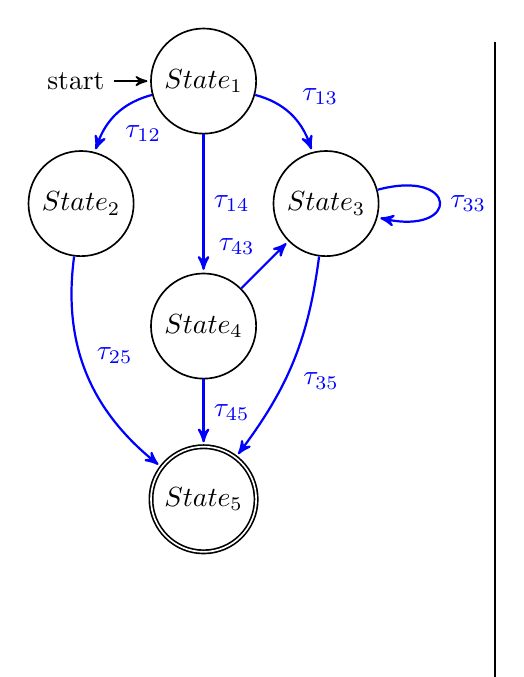
\begin{tikzpicture}[>=stealth', shorten >=1pt, auto, node distance=2.2cm, semithick,
													dot/.style={circle,inner sep=1pt,fill,label={#1},name=#1},
		  										extended line/.style={shorten >=-#1,shorten <=-#1},
		  										extended line/.default=1cm,
		  										block/.style={rectangle,draw, text centered, rounded corners, minimum height=4em, minimum width=12em}]
		  										
			  \tikzstyle{every state}=[fill=white, draw=black, text=black]
			
			  \node[initial,state] (A)                    {$State_{1}$};
			  \node[state]         (B) [below left of=A]  {$State_{2}$};
			  \node[state]         (C) [below right of=A] {$State_{3}$};
			  \node[state]         (D) [below left of=C]  {$State_{4}$};
			  \node[state,accepting]  (E) [below of=D]       {$State_{5}$};
		
			  \path[->,thick] (A) edge [blue, bend right]      node {$\tau_{12}$} (B)
			                      edge [blue, bend left]       node {$\tau_{13}$} (C)
			                      edge [blue]                  node {$\tau_{14}$} (D)
								        (B) edge [blue, bend right]      node {$\tau_{25}$} (E)
								        (C) edge [blue, bend left=15pt]  node {$\tau_{35}$} (E)
								            edge [blue, loop right]      node {$\tau_{33}$} (C)
								        (D) edge [blue]                  node {$\tau_{43}$} (C)
								        (D) edge [blue]                  node {$\tau_{45}$} (E);
								        
				\draw [thick, extended line=1cm] (3.7,-0.5) -- (3.7,-7.2);
				
			\end{tikzpicture}
    \end{minipage}
    \hspace{0.5cm}
    \begin{minipage}[h]{0.5\linewidth}
      \caption{High-level description of the test program}\label{verb:hl-desc}
      \centering
      \lstset{basicstyle=\scriptsize,tabsize=2}
			\begin{lstlisting}
    State1: Par = receive()
            Vreader = receive()
            Vnvm = read(nvm)
            if(Vreader == Vnvm)
    State2:    par = (par)^2
               goto State5
            end
            else if(Vreader > Vnvm)
    State4:    par = par + 216
               par = par/5
               Vreader = Vreader - 2
               if(Vreader < Vnvm)
                  goto State3
               end
               else
                  goto State5
               end
            end
            else if(Vreader < Vnvm)
    State3:    par = par * 2
               par = par - 129
               Vreader = Vreader + 1
               if (Vreader < Vnvm)
                  goto State3
               end
               else
                  goto State5
               end
            end
    State5: clear_registers
            clear_memory
				\end{lstlisting}
    \end{minipage}
\end{figure*}

Invoking the test program requires passing two arguments: ``$V_{reader}$'' ($0\leq V_{reader}\leq 9$) and ``$Par$'' ($0\leq Par\leq 255$). The ``$V_{reader}$'' is compared with a reference value ``$V_{nvm}$'' ($0\leq V_{nvm}\leq 9$) (stored in the non-volatile memory of the smart card) before changing a state. For our experiment the $V_{nvm}$ is initialised to ``4'' and the arguments $Par$ and $V_{reader}$ are randomly generated and passed to the program through the smart card reader.

\subsubsection{Building The Hidden Markov Model}
\label{subsubsec:exp-hmm}

As discussed in Section~\ref{subsubsec:build-hmm}, building a \emph{Hidden Markov Model} requires the initial probability distribution $\vec{\pi}$, transition probability distribution $\mathbf{T}$ and the emission probability distribution $\mathbf{E}$. As illustrated in Fig.~\ref{fig:test-app}, the execution of the test program always starts at $State_{1}$. Therefore, the probability of $State_{1}$ being the initial state is ``1'', and ``0'' for all other states. If $\pi_{i}$ is the probability of $State_{i}$ being the initial state in the execution of the program, the initial probability distribution vector of our test program is given as:

\begin{equation}
	\vec{\pi} = \{ \begin{array}{ccccc} \pi_1 = 1, & \pi_2 = 0, & \pi_3 = 0, & \pi_4 = 0, & \pi_5 = 0 \end{array} \}
	\label{equ:intial-pro-dist}
\end{equation}

To compute the transition probability distribution matrix, $\mathbf{T}$, we invoked the program with a randomly generated ``$Par$'' and all possible values (i.e. $0$ to $9$) of ``$V_{reader}$'' and record the control-flow transition of the program. Note that for each different value of ``$V_{nvm}$'' the matrix $\mathbf{T}$ is different.

\begin{table}
	\centering
	\caption{Transition probability distribution of the program illustrated in Fig.~\ref{fig:test-app} and \ref{verb:hl-desc}. The columns represent next states and the rows represent current states.}
	\begin{tabular*}{\textwidth}{c@{\extracolsep{\fill}}|cccccc}
	\hline
	\textbf{Transition from} & \multicolumn{5}{c}{\textbf{Transition to [\%]}} \\
	
			                     & $State_{1}$     & $State_{2}$       & $State_{3}$       & $State_{4}$       & $State_{5}$      \\
	 \hline
	 $State_{1}$             &  $\tau_{11}$=0  &  $\tau_{12}$=0.1  &  $\tau_{13}$=0.4  &  $\tau_{14}$=0.5  &  $\tau_{15}$=0   \\
	 $State_{2}$             &  $\tau_{21}$=0  &  $\tau_{22}$=0    &  $\tau_{23}$=0    &  $\tau_{24}$=0    &  $\tau_{25}$=1   \\
	 $State_{3}$             &  $\tau_{31}$=0  &  $\tau_{32}$=0    &  $\tau_{33}$=0.55 &  $\tau_{34}$=0    &  $\tau_{35}$=0.45\\
	 $State_{4}$             &  $\tau_{41}$=0  &  $\tau_{42}$=0    &  $\tau_{43}$=0.2  &  $\tau_{44}$=0    &  $\tau_{45}$=0.8 \\
	 $State_{5}$             &  $\tau_{51}$=0  &  $\tau_{52}$=0    &  $\tau_{53}$=0    &  $\tau_{54}$=0    &  $\tau_{55}$=0   \\
	 \hline
	
	\end{tabular*}
	\label{tbl:tpd}
\end{table}

To compute the emission probability distribution matrix $\mathbf{E}$, we collected 1000 traces for each state. Using these traces we computed the mean $\mu_{q_{i}}$, and covariance, $\sigma_{q_{i}}$, for each state as a template.

\begin{figure*}[h]
\centering
	\begin{tikzpicture}
	  \begin{groupplot}[group style = {
	  										group size = 1 by 5,
	  										xlabels at = edge bottom,
	        							xticklabels at = edge bottom,
	  										vertical sep = 0pt
	  									},
									    grid = major,
									    footnotesize,
									    width = 10cm,
									    height =1.2cm,
									    scale only axis,
									    xmin = 1,
									    xmax = 1600,
									    xtick = {0, 250, 375, 875, 1000, 1250},
									    xticklabels = {0,250, 375, 875, 1000, 1250},
									    xlabel = {Trace Samples},
											ylabel = {mV},
									    ymin = -0.2,
									    ytick align = outside,
	    								xtick align = outside,
									    ymax = 0.3,
									    unbounded coords = jump
			]
	    
		    \nextgroupplot
		    \addplot plot[smooth, thick, mark=*, thick, mark size=0pt, green] file{state_one.dat};
		    \legend{$State_{1}$\\}
		    \nextgroupplot
		    \addplot plot[smooth, thick, mark=*, thick, mark size=0pt, magenta] file{state_two.dat};
		    \legend{$State_{2}$\\}
		    \nextgroupplot
		    \addplot plot[smooth, thick, mark=*, thick, mark size=0pt, cyan] file{state_three.dat};
		    \legend{$State_{3}$\\}
		    \nextgroupplot
		    \addplot plot[smooth, thick, mark=*, thick, mark size=0pt, black] file{state_four.dat};
		    \legend{$State_{4}$\\}
		    \nextgroupplot
		    \addplot plot[smooth, thick, mark=*, thick, mark size=0pt, gray] file{state_five.dat};
		    \legend{$State_{5}$\\}
	  \end{groupplot}
	\end{tikzpicture}
	\caption{Mean of the power traces of the states illustrated in Fig.~\ref{fig:test-app}.}\label{fig:state-power-consumption}
\end{figure*}

As shown in figure~\ref{fig:state-power-consumption}, the states of the test application generate power consumption traces of different dimension. In our experiment $\mathbf{E}$ is computed over the first 250 sample points of the traces. However, a covariance matrix of $250\times 250$ is still too large to compute its inverse. For this purpose we applied the techniques discussed in Section~\ref{subsubsec:build-hmm} (PCA and F-LDA) on the first 250 sample points of the state emission (power consumption) before computing $\mathbf{E}$.

\paragraph{\textbf{Principal Components Analysis (PCA)}} is used to find a subspace whose basis vectors corresponding to the maximum variance directions in the original data. In other words PCA searches for those vectors in the underlying data that best describes the data. When applying \emph{PCA} the dimensionality of the projected data has to be selected carefully. On the one hand, if it is too small, too much of variance of the original data may get lost and with it important information about the state emissions. On the other hand, if it is too large, the state classification becomes less reliable again. This might be because of the bad conditioning of large covariance matrix. Another reason can be, as the dimension increase the class emission cross-correlation increases. Therefore, when choosing the dimensionality for the projected data we have to decide how much of variance of the original data that we can afford to lose. 

\begin{figure}[h]
	\centering
	\begin{tikzpicture}
		\begin{axis}[
			xlabel={First Principal Component},
			ylabel={Second Principal Component},
			width=\textwidth,
			height=2.3in,
			xmin=-0.35, xmax=0.35,
			ymin=-0.15, ymax=0.15,
			legend pos= north west]
				\addplot plot[mark=*, mark size=1pt, only marks, green] file{state_data_pca/state_1_pca.dat};
				\addplot plot[mark=*, mark size=1pt, only marks, magenta] file{state_data_pca/state_2_pca.dat};
				\addplot plot[mark=*, mark size=1pt, only marks, cyan] file{state_data_pca/state_3_pca.dat};
				\addplot plot[mark=*, mark size=1pt, only marks, black] file{state_data_pca/state_4_pca.dat};
				\addplot plot[mark=*, mark size=1pt, only marks, gray] file{state_data_pca/state_5_pca.dat};
	    	\legend{$State_{1}$\\$State_{2}$\\$State_{3}$\\$State_{4}$\\$State_{5}$\\}
  	\end{axis}
	\end{tikzpicture}
	\caption{Original data after PCA.}\label{fig:state-data-pca}
\end{figure}

For example, in our experiment the first 100 principal components were accounted for 54.76\% of variance of the original emission. the first 250 principal components are accounted for 80.74\% of variance of the original emission. In Fig.\ref{fig:state-data-pca} we show plots of the first two principal components after PCA.

\paragraph{\textbf{Fisher's Linear Discriminant Analysis (F-LDA)}} is a technique used to classify between classes by finding discriminant features of the class data and projecting them onto these discriminant vectors. In other words, F-LDA searches for those vectors in the underlying data that best separates among the classes.

\begin{figure}[h]
	\centering
	\begin{tikzpicture}
		\begin{axis}[
			xlabel={First LDA Component},
			ylabel={Second LDA Component},
			width=\textwidth,
			height=2.3in,
			xmin=-0.35, xmax=0.35,
			ymin=-0.15, ymax=0.15,
			legend pos= north east]
				\addplot plot[mark=*, mark size=1pt, only marks, green] file{state_data_lda/state_1_lda.dat};
				\addplot plot[mark=*, mark size=1pt, only marks, magenta] file{state_data_lda/state_2_lda.dat};
				\addplot plot[mark=*, mark size=1pt, only marks, cyan] file{state_data_lda/state_3_lda.dat};
				\addplot plot[mark=*, mark size=1pt, only marks, black] file{state_data_lda/state_4_lda.dat};
				\addplot plot[mark=*, mark size=1pt, only marks, gray] file{state_data_lda/state_5_lda.dat};
	    	\legend{$State_{1}$\\$State_{2}$\\$State_{3}$\\$State_{4}$\\$State_{5}$\\}
  	\end{axis}
	\end{tikzpicture}
	\caption{Original data after F-LDA.}\label{fig:state-data-lda}
\end{figure}

In Fig.~\ref{fig:state-data-lda} we present the first two components of the state emissions after F-LDA. As discussed earlier PCA searches for vectors that best describes the original data. However, it does not take the other classes into consideration. For this reason PCA may not produce a satisfactory result when classifying different classes. We can see that in Fig.~\ref{fig:state-data-pca} the principal components of classes emissions overlap. However, as shown in Fig.~\ref{fig:state-data-lda} the classes are better separated after F-LDA.

\subsubsection{Calculating The Most Probable State Sequence}
\label{subsec:exp-viterbi}

To calculate the most probable state sequence, first we have to implement the \emph{Viterbi Algorithm} discussed in Section~\ref{subsubsec:state-seq}. To do this we have two options: use the MATLAB \cite{matlab} Statistics Toolbox implementation \emph{hmmviterbi}\cite{hmm-viterbi} or create our own implementation of the equations~(\ref{equ:viterbi-init}) and~(\ref{equ:viterbi}). Although, the MATLAB Statistics Toolbox implementation of \emph{Viterbi Algorithm} might be useful for some statistical calculations we could not use it in our experiment. This was because firstly it does not utilise the initial probability distribution ($\vec{\pi}$) and secondly the output is not in the format that we want it to be. Therefore, we created our own MATLAB implementation and the source code is available at the end of the paper in Appendix~\ref{sec:viterbi-implementation}. As you can see it from the source code, our implementation takes all three matrices ($\vec{\pi}$, $\mathbf{E}$ and $\mathbf{T}$) that we discussed in Section~\ref{sec:control-flow-verification} and gives us the most likely state sequence as a vector.

Our test program has six valid control-flow paths from the initial state, $state_{1}$, to the final state, $state_{5}$. Our implementation of the \emph{Viterbi algorithm} calculates a sequence of states with the highest probability of generating the emission $\mathcal{O}$. We ran the test program for all possible valid paths by varying the argument ``$V_{reader}$'' and calculated the most probable state sequence from the smart cards power consumption trace. We ran the test program 1000 times by varying ``$V_{Reader}$'', recorded the power trace and calculated the most likely sequence of states for each run.

\subsection{Verifying The Reconstructed State Sequence}
\label{subsec:exp-verify}

For all the state sequences that we calculated, we verified them using the 2-step verification system discussed in Section~\ref{subsec:verification}. Before comparing the reconstructed state sequence against the CFG, we have to make sure that the reconstructed sequence is the actual path that the smart card went through. For that purpose we verified the hash values calculated by the smart card against the hash values calculated over the reconstructed state sequence. Then we compared the reconstructed state sequence against the valid paths in CFG. In our experiment we successfully verified the control flow for all (1000) runs of the test program that we made. In our experiment we calculated the CFG manually; however, for large programs calculating it manually might be difficult and complicated. In such a case the CFG may be extracted using a source code analysis tools, such as MALPAS \cite{malpas}. 

\section{Conclusion}
\label{sec:conclusion}

In the literature several methods have been proposed to counteract a program's control flow violation. In most of them the proposed solutions require either a dedicated hardware module or the main processor to perform extra computations to check the control flow security of the program(s) at runtime. Usually this computation utilises the program's properties which are extracted ahead of time, such as CFG. These properties are then used to check the program's behaviour dynamically. However, these kind of solutions may not be suitable for low-end devices deployed as coprocessors in bigger systems, such as hardware security modules in communication devices.

In this paper we proposed a novel approach into checking a program's control flow integrity by using the side channel leakage of the target device. In our method the device is not required to perform extra computation. However, it requires another device to check for its program's control flow integrity as it executes the program. This method can be used in smart card (or any other embedded device that need to connect to an external device to execute the application) where the terminal (external device) acts as the verifying device.

\bibliographystyle{unsrt}
\bibliography{./reference}

\appendix

\section*{Appendix}

\section{Viterbi MATLAB Implementation}
\label{sec:viterbi-implementation}



\lstset{basicstyle=\small\ttfamily,
				numbersep=1pt,
				keywordstyle=\color{blue}\textbf,
				commentstyle=\color{commentColor}\textit,
				language=Matlab,
				breaklines=true,
				caption=MATLAB implementation of the Viterbi algorithm described in section~\ref{subsubsec:state-seq}}
\lstinputlisting{viterbi_matlab/viterbi_sequence.m}

\end{document}
